\chapter{Ion dan Larutan Ion}\label{ch:g9:ions}

Dua minuman jernih berdiri di atas bangku olahraga: sebotol minuman
isotonik, yang dijual karena ``elektrolit''-nya, dan segelas air gula.
Di laboratorium, dua lempeng logam yang dihubungkan ke baterai dan
sebuah bola lampu kecil dicelupkan bergantian ke dalam masing-masing
minuman. Dalam minuman isotonik, lampu menyala; dalam air gula, lampu
tetap padam. Ada sesuatu dalam cairan pertama yang membawa muatan
listrik, dan gula tidak. Sesuatu itu adalah \omterm{def:g9:ions:ion}{ion}.

\begin{recall}
Sebuah \omterm{def:g7:atoms-and-molecules:atom}{atom} memiliki inti dengan $Z$ \omterm{def:g9:inside-the-atom:proton}{proton}, masing-masing bermuatan
$+e$, dan $Z$ \omterm{def:g9:inside-the-atom:nucleus}{elektron} di sekelilingnya, masing-masing bermuatan $-e$:
\omterm{def:g7:atoms-and-molecules:atom}{atom} itu netral (\cref{ch:g9:inside-the-atom}). \omterm{def:g6:solutions-and-solubility:solute}{Zat terlarut} yang \omterm{def:g2:mixing-and-dissolving:dissolve}{larut}
dalam air menghasilkan \omterm{def:g6:solutions-and-solubility:solute}{larutan berair}
(\cref{ch:g6:solutions-and-solubility}). \omterm{def:g7:identifying-substances:characteristic-test}{Uji khas} mendeteksi suatu
spesies melalui hasil yang terlihat
(\cref{ch:g7:identifying-substances}).
\end{recall}

\begin{omfigure}
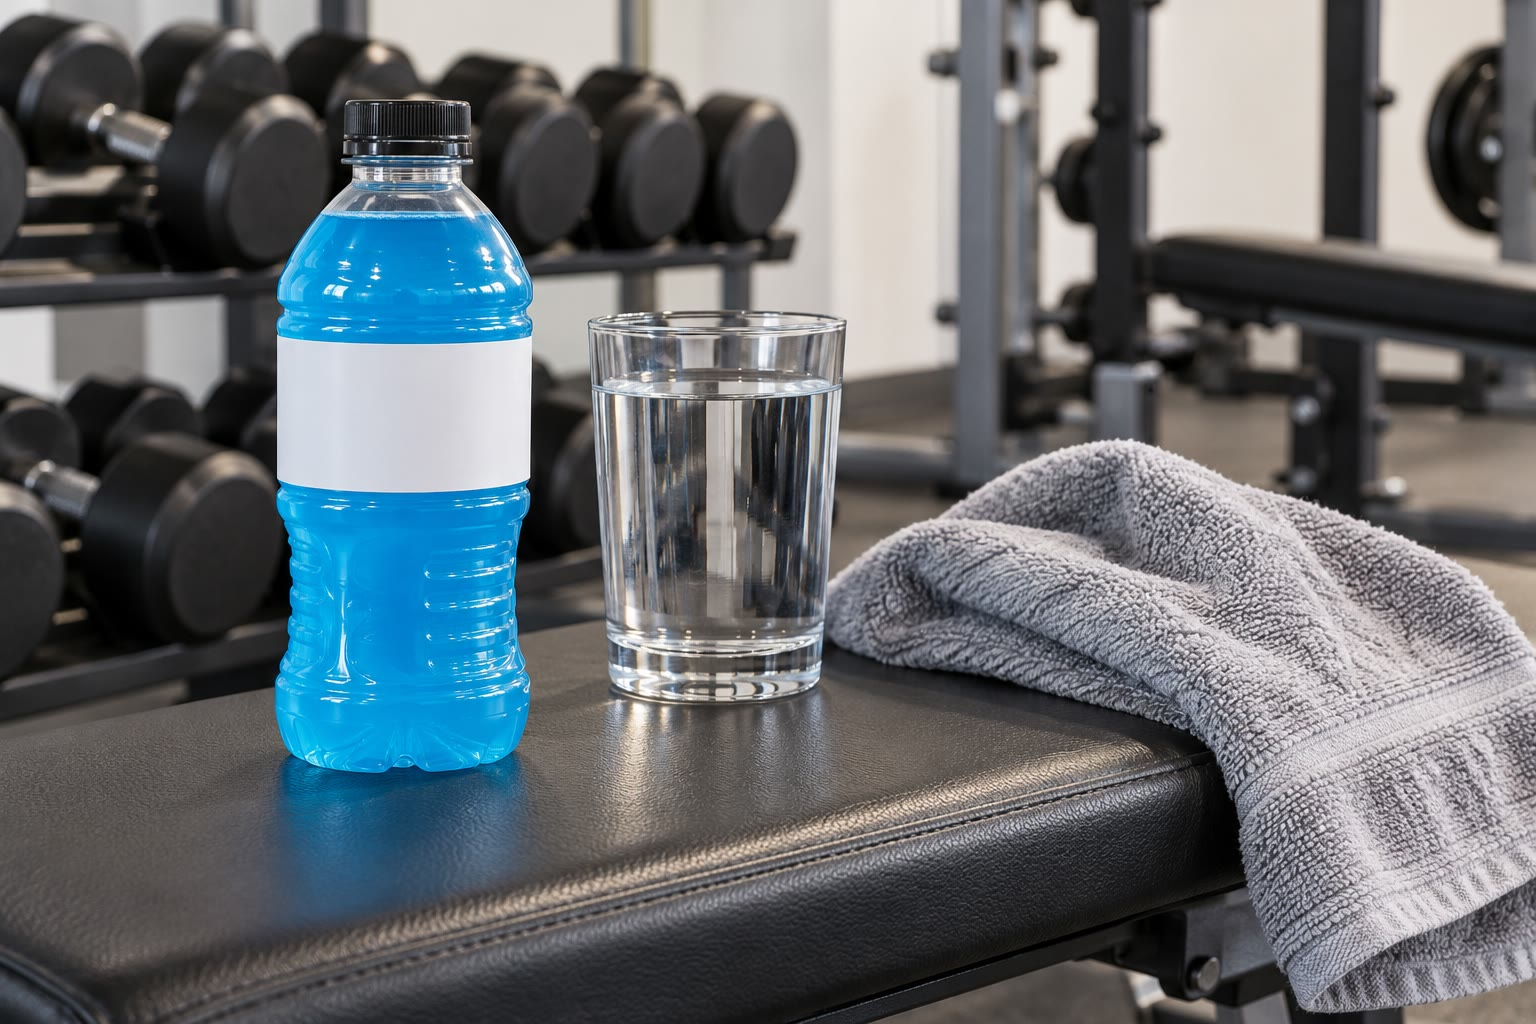
\includegraphics[width=0.5\linewidth]{images/book1/ai/g9-sports-drink.jpg}

{\small Minuman isotonik dan segelas air: minuman itu mengandung
\omterm{def:g9:ions:ion}{ion-ion} terlarut.}
\end{omfigure}

\section{Atom yang menerima atau melepaskan elektron}

\begin{definition}[Ion, kation, anion]\label{def:g9:ions:ion}
Sebuah \emph{ion}\index{ion} adalah \omterm{def:g7:atoms-and-molecules:atom}{atom}, atau sekelompok \omterm{def:g7:atoms-and-molecules:atom}{atom}, yang
telah melepaskan atau menerima satu \omterm{def:g9:inside-the-atom:nucleus}{elektron} atau lebih, sehingga
bermuatan listrik. Ion yang bermuatan positif, karena telah melepaskan
\omterm{def:g9:inside-the-atom:nucleus}{elektron}, disebut \emph{kation}\index{kation}; ion yang bermuatan
negatif, karena telah menerima \omterm{def:g9:inside-the-atom:nucleus}{elektron}, disebut
\emph{anion}\index{anion}. Muatannya ditulis di kanan atas rumus:
\ce{Na+}, \ce{Cu^{2+}}, \ce{Cl-}.
\end{definition}

\begin{example}[Natrium dan klorin]\label{ex:g9:ions:na-cl}
Sebuah \omterm{def:g7:atoms-and-molecules:atom}{atom} natrium, 11 \omterm{def:g9:inside-the-atom:proton}{proton} dan 11 \omterm{def:g9:inside-the-atom:nucleus}{elektron}, melepaskan satu
\omterm{def:g9:inside-the-atom:nucleus}{elektron}: \omterm{def:g7:atoms-and-molecules:atom}{atom} itu menjadi \omterm{def:g9:ions:ion}{ion} natrium \ce{Na+}, 11 \omterm{def:g9:inside-the-atom:proton}{proton} dan 10
\omterm{def:g9:inside-the-atom:nucleus}{elektron}, bermuatan $+1$:
\[
  \ce{Na -> Na+ + e-}.
\]
Sebuah \omterm{def:g7:atoms-and-molecules:atom}{atom} klorin, 17 \omterm{def:g9:inside-the-atom:proton}{proton} dan 17 \omterm{def:g9:inside-the-atom:nucleus}{elektron}, menerima satu \omterm{def:g9:inside-the-atom:nucleus}{elektron}:
\omterm{def:g7:atoms-and-molecules:atom}{atom} itu menjadi \omterm{def:g9:ions:ion}{ion} klorida \ce{Cl-}, 17 \omterm{def:g9:inside-the-atom:proton}{proton} dan 18 \omterm{def:g9:inside-the-atom:nucleus}{elektron}:
\[
  \ce{Cl + e- -> Cl-}.
\]
\end{example}

\begin{omfigure}
\begin{tikzpicture}[font=\small]
  \foreach \x/\name/\p/\e/\ch/\col in {0/{atom natrium}/11/11/0/omDef,
      3.7/{ion natrium \ce{Na+}}/11/10/+1/omProp,
      8.0/{atom klorin}/17/17/0/omDef, 11.7/{ion klorida \ce{Cl-}}/17/18/$-1$/omProp} {
    \node[draw=\col, fill=\col!6, rounded corners=2pt, align=center, text width=2.4cm]
      at (\x,0) {\textbf{\name}\\ \p\ proton\\ \e\ elektron\\ muatan \ch};
  }
  \draw[->, thick, omProp] (1.45,0) -- (2.25,0) node[midway, above, text=black,
    font=\footnotesize, align=center] {melepas\\ 1 \ce{e-}};
  \draw[->, thick, omProp] (9.45,0) -- (10.25,0) node[midway, above, text=black,
    font=\footnotesize, align=center] {menerima\\ 1 \ce{e-}};
\end{tikzpicture}

{\small Sebuah \omterm{def:g7:atoms-and-molecules:atom}{atom} natrium menjadi \omterm{def:g9:ions:ion}{ion} natrium dengan melepaskan satu
\omterm{def:g9:inside-the-atom:nucleus}{elektron}; sebuah \omterm{def:g7:atoms-and-molecules:atom}{atom} klorin menjadi \omterm{def:g9:ions:ion}{ion} klorida dengan menerima satu
\omterm{def:g9:inside-the-atom:nucleus}{elektron}. \omterm{def:g9:inside-the-atom:proton}{Protonnya} tidak berubah.}
\end{omfigure}

\begin{proposition}[Beberapa ion yang umum]\label{prop:g9:ions:common}
\omterm{def:g9:ions:ion}{Ion} monoatomik terbentuk dari satu \omterm{def:g7:atoms-and-molecules:atom}{atom}; \omterm{def:g9:ions:ion}{ion} poliatomik dari sekelompok
\omterm{def:g7:atoms-and-molecules:atom}{atom} yang tetap bersatu:
\begin{center}
\small
\begin{tabular}{llll}
\hline
\omterm{def:g9:ions:ion}{kation} & & \omterm{def:g9:ions:ion}{anion} & \\
\hline
natrium & \ce{Na+} & klorida & \ce{Cl-} \\
kalium & \ce{K+} & hidroksida & \ce{OH-} \\
kalsium & \ce{Ca^{2+}} & nitrat & \ce{NO3-} \\
magnesium & \ce{Mg^{2+}} & karbonat & \ce{CO3^{2-}} \\
tembaga(II) & \ce{Cu^{2+}} & sulfat & \ce{SO4^{2-}} \\
besi(II), besi(III) & \ce{Fe^{2+}}, \ce{Fe^{3+}} & & \\
seng & \ce{Zn^{2+}} & & \\
aluminium & \ce{Al^{3+}} & & \\
amonium & \ce{NH4+} & & \\
\hline
\end{tabular}
\end{center}
\end{proposition}

\section{Senyawa ion dan rumusnya}

\begin{definition}[Senyawa ion]\label{def:g9:ions:ionic-compound}
Sebuah \emph{senyawa ion}\index{senyawa ion} tersusun atas \omterm{def:g9:ions:ion}{kation} dan
\omterm{def:g9:ions:ion}{anion} dalam jumlah sedemikian rupa sehingga keseluruhannya tidak
bermuatan. Rumusnya menyatakan perbandingan \omterm{def:g9:ions:ion}{ion-ionnya}, tanpa
muatannya: \ce{NaCl} untuk natrium klorida, satu \ce{Na+} untuk setiap
\ce{Cl-}; \ce{CaCl2} untuk kalsium klorida, dua \ce{Cl-} untuk setiap
\ce{Ca^{2+}}.
\end{definition}

\begin{method}[Menuliskan rumus senyawa ion]\label{met:g9:ions:formula}
\begin{enumerate}
  \item Tuliskan kedua \omterm{def:g9:ions:ion}{ion} dengan muatannya, \omterm{def:g9:ions:ion}{kation} lebih dulu.
  \item Tentukan jumlah terkecil masing-masing \omterm{def:g9:ions:ion}{ion} yang membuat muatan
        totalnya nol.
  \item Tuliskan jumlah-jumlah itu sebagai \omterm{def:g7:atoms-and-molecules:formula}{angka indeks}; \omterm{def:g9:ions:ion}{ion} poliatomik
        yang memerlukan \omterm{def:g7:atoms-and-molecules:formula}{angka indeks} ditulis di dalam tanda kurung.
\end{enumerate}
Aluminium oksida: \ce{Al^{3+}} dan \ce{O^{2-}}; $2 \times (+3) + 3 \times
(-2) = 0$, jadi \ce{Al2O3}. Besi(III) hidroksida: \ce{Fe^{3+}} dan tiga
\ce{OH-}: \ce{Fe(OH)3}.
\end{method}

\begin{proposition}[Padatan ion adalah tumpukan ion]\label{prop:g9:ions:solid}
Dalam sebutir kristal garam, \omterm{def:g9:ions:ion}{ion} natrium dan \omterm{def:g9:ions:ion}{ion} klorida berselang-seling
dalam tumpukan tiga dimensi yang teratur, setiap \omterm{def:g9:ions:ion}{ion} dikelilingi oleh
\omterm{def:g9:ions:ion}{ion-ion} yang muatannya berlawanan, yang menahannya di tempatnya.
Sebutir garam dapur mengandung miliaran miliar \omterm{def:g9:ions:ion}{ion}; bentuknya yang
kubus mencerminkan tumpukan yang berbentuk kubus itu.
\end{proposition}

\begin{omfigure}
\begin{minipage}[b]{0.5\linewidth}\centering
\begin{tikzpicture}[font=\small]
  \foreach \i in {0,...,5} \foreach \j in {0,...,4} {
    \pgfmathtruncatemacro\pp{mod(\i+\j,2)}
    \ifnum\pp=0 \node[aNa, minimum size=5mm] at (0.62*\i,0.62*\j) {};
    \else \node[aCl, minimum size=7.4mm] at (0.62*\i,0.62*\j) {};\fi
  }
\end{tikzpicture}

{\small Satu lapisan kristal garam: \omterm{def:g9:ions:ion}{ion} natrium (ungu, lebih kecil) dan
\omterm{def:g9:ions:ion}{ion} klorida (hijau) berselang-seling.}
\end{minipage}\hfill
\begin{minipage}[b]{0.3\linewidth}\centering
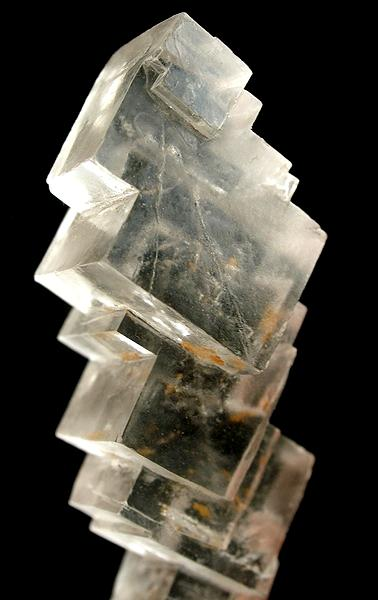
\includegraphics[height=4.6cm]{images/book1/halite.jpg}

{\small Halit, garam batu alami. Foto: Robert M.~Lavinsky,
CC\ BY-SA\ 3.0.}
\end{minipage}
\end{omfigure}

\section{Larutan ion menghantarkan listrik}

\begin{notation}[Lambang wujud (aq)]\label{not:g9:ions:aq}
\omterm{def:g9:ions:ion}{Ion} atau \omterm{def:g7:atoms-and-molecules:molecule}{molekul} yang \omterm{def:g2:mixing-and-dissolving:dissolve}{larut} dalam air ditandai (aq), dari kata Latin
\textit{aqua}, air: \ce{Na+(aq)}, \ce{Cl-(aq)}.
\end{notation}

\begin{proposition}[Larutan ion menghantarkan listrik]\label{prop:g9:ions:conduct}
Ketika sebuah \omterm{def:g9:ions:ionic-compound}{senyawa ion} \omterm{def:g2:mixing-and-dissolving:dissolve}{larut} dalam air, \omterm{def:g9:ions:ion}{ion-ionnya} terpisah dan
bergerak bebas di dalam larutan: air garam mengandung \ce{Na+(aq)} dan
\ce{Cl-(aq)}. \omterm{def:g9:ions:ion}{Ion} yang bergerak membawa muatan listrik, sehingga larutan
\omterm{def:g9:ions:ion}{ion} menghantarkan listrik. Larutan gula, yang \omterm{def:g7:atoms-and-molecules:molecule}{molekulnya} tidak
bermuatan, tidak menghantarkan listrik; begitu pula air yang sangat
murni.
\end{proposition}

\begin{inthelab}[Cairan mana yang menghantarkan listrik?]
Guru merangkai dua lempeng logam, sebuah baterai bertegangan rendah,
dan sebuah bola lampu kecil menjadi satu rangkaian; lempeng-lempeng itu
dicelupkan bergantian ke dalam air suling, air gula, air garam, dan
larutan tembaga sulfat, dan dibilas setiap kali. Lampu hanya menyala
dengan kedua larutan \omterm{def:g9:ions:ion}{ion}.
\end{inthelab}

\begin{omfigure}
\begin{tikzpicture}[font=\small, scale=1.1]
  \foreach \xs/\lit/\lab in {0/1/{air garam: lampu menyala}, 5.2/0/{air gula: lampu tetap padam}} {
    \begin{scope}[xshift=\xs cm]
      \pic[transform shape] at (2,0) {beaker={0.7}{omWater!80}};
      \fill[black!45] (1.6,0.25) rectangle (1.7,2.6);
      \fill[black!45] (2.3,0.25) rectangle (2.4,2.6);
      \ifnum\lit=1 \fill[yellow!70, opacity=0.8] (3.4,3.0) circle (0.42);\fi
      \draw (1.65,2.6) -- (1.65,3.6) to[battery1] (3.4,3.6) -- (3.4,3.4)
        to[lamp] (3.4,2.6) -- (2.35,2.6);
      \node[anchor=north, align=center] at (2,-0.15) {\lab};
    \end{scope}
  }
\end{tikzpicture}

{\small Uji daya hantar: dengan air garam, \omterm{def:g9:ions:ion}{ion-ion} membawa arus dan
lampu menyala; air gula tidak mengandung \omterm{def:g9:ions:ion}{ion} dan lampu tetap padam.}
\end{omfigure}

\section{Uji pengendapan untuk ion}

\begin{definition}[Endapan]\label{def:g9:ions:precipitate}
Ketika dua larutan \omterm{def:g2:mixing-and-dissolving:mix}{dicampur}, \omterm{def:g9:ions:ion}{kation} dari larutan yang satu dan \omterm{def:g9:ions:ion}{anion}
dari larutan yang lain dapat membentuk \omterm{def:g9:ions:ionic-compound}{senyawa ion} yang tidak \omterm{def:g2:mixing-and-dissolving:dissolve}{larut}.
Senyawa itu muncul sebagai padatan halus yang mengeruhkan cairan lalu
mengendap: sebuah \emph{endapan}\index{endapan}. Reaksinya disebut
\emph{reaksi pengendapan}\index{reaksi pengendapan}.
\end{definition}

\begin{proposition}[Uji untuk ion-ion yang umum]\label{prop:g9:ions:tests}
Beberapa tetes larutan \omterm{def:g7:identifying-substances:characteristic-test}{reagen} mengenali sebuah \omterm{def:g9:ions:ion}{ion} dari warna \omterm{def:g9:ions:precipitate}{endapan}
yang dibentuknya:
\begin{center}
\small
\begin{tabular}{llll}
\hline
\omterm{def:g9:ions:ion}{ion} yang dicari & \omterm{def:g7:identifying-substances:characteristic-test}{reagen} & \omterm{def:g9:ions:precipitate}{endapan} & warna \\
\hline
tembaga(II) \ce{Cu^{2+}} & natrium hidroksida & \ce{Cu(OH)2} & biru \\
besi(II) \ce{Fe^{2+}} & natrium hidroksida & \ce{Fe(OH)2} & hijau \\
besi(III) \ce{Fe^{3+}} & natrium hidroksida & \ce{Fe(OH)3} & jingga kecokelatan \\
seng \ce{Zn^{2+}} & natrium hidroksida & \ce{Zn(OH)2} & putih \\
aluminium \ce{Al^{3+}} & natrium hidroksida & \ce{Al(OH)3} & putih \\
klorida \ce{Cl-} & perak nitrat & \ce{AgCl} & putih, menggelap di bawah cahaya \\
\hline
\end{tabular}
\end{center}
\end{proposition}

\begin{example}[Menuliskan reaksi pengendapan]\label{ex:g9:ions:equation}
Hanya \omterm{def:g9:ions:ion}{ion-ion} yang membentuk padatan yang dituliskan; \omterm{def:g9:ions:ion}{ion-ion} lainnya
tetap terlarut dan tidak ikut bereaksi:
\[
  \ce{Cu^{2+}(aq) + 2OH-(aq) -> Cu(OH)2(s)}, \qquad
  \ce{Ag+(aq) + Cl-(aq) -> AgCl(s)}.
\]
\end{example}

\begin{omfigure}
\begin{tikzpicture}[font=\small, scale=0.95]
  \foreach \k/\pc/\lab in {0/blue!60/{\ce{Cu^{2+}}: biru}, 1/green!45!black!70/{\ce{Fe^{2+}}: hijau},
      2/orange!70!brown/{\ce{Fe^{3+}}: jingga\\kecokelatan}, 3/white!85!black/{\ce{Zn^{2+}}: putih},
      4/white!85!black/{\ce{Al^{3+}}: putih}, 5/white!80!black/{\ce{Cl-}: putih}} {
    \pic[transform shape] at (\k*2.3,0) {testtube={0.5}{omWater!60}};
    \pic[transform shape] at (\k*2.3,0) {testtube={0.14}{\pc}};
    \node[anchor=north, align=center, font=\footnotesize, text width=2cm] at (\k*2.3,-0.15) {\lab};
  }
\end{tikzpicture}

{\small \omterm{def:g9:ions:precipitate}{Endapan} yang terbentuk dengan natrium hidroksida (lima tabung
pertama) dan dengan perak nitrat (tabung terakhir).}
\end{omfigure}

\begin{safety}{\ghs[0.82cm]{GHS05}\ghs[0.82cm]{GHS07}}
% ledger: ghs:NaOH, ghs:AgNO3
Natrium hidroksida: menyebabkan luka bakar kulit dan kerusakan mata yang
parah, dan dapat bersifat korosif terhadap logam (GHS05); dalam bentuk
encer menyebabkan iritasi kulit dan mata (GHS07). Perak nitrat, \omterm{def:g7:identifying-substances:characteristic-test}{reagen}
untuk klorida, adalah oksidator, korosif, dan sangat beracun bagi
kehidupan akuatik. Pakai kacamata pelindung dan sarung tangan; \omterm{def:g7:identifying-substances:characteristic-test}{reagen}
diteteskan oleh guru.
\end{safety}

\begin{method}[Menguji sebuah ion]\label{met:g9:ions:test}
\begin{enumerate}
  \item Tuang sedikit larutan yang akan diuji ke dalam tabung reaksi.
  \item Tambahkan \omterm{def:g7:identifying-substances:characteristic-test}{reagennya} tetes demi tetes.
  \item Catat warna \omterm{def:g9:ions:precipitate}{endapan} yang terbentuk, lalu bandingkan dengan tabel.
  \item Simpulkan, dan ingatlah bahwa sebuah uji mengenali \omterm{def:g9:ions:ion}{ion}, bukan
        senyawa: larutan besi(III) klorida memberikan hasil positif baik
        pada uji \ce{Fe^{3+}} maupun pada uji \ce{Cl-}.
\end{enumerate}
\end{method}

\section{Latihan}

\begin{exercise}[$\star$]\label{exo:g9:ions:1}
Apa itu \omterm{def:g9:ions:ion}{ion}? Apa perbedaan antara \omterm{def:g9:ions:ion}{kation} dan \omterm{def:g9:ions:ion}{anion}?
\end{exercise}

\begin{exercise}[$\star$]\label{exo:g9:ions:2}
Sebuah \omterm{def:g7:atoms-and-molecules:atom}{atom} magnesium (12 \omterm{def:g9:inside-the-atom:proton}{proton}) melepaskan dua \omterm{def:g9:inside-the-atom:nucleus}{elektron}. Tuliskan
rumus \omterm{def:g9:ions:ion}{ion} yang terbentuk, dan berikan banyaknya \omterm{def:g9:inside-the-atom:proton}{proton} dan \omterm{def:g9:inside-the-atom:nucleus}{elektronnya}.
\end{exercise}

\begin{exercise}[$\star$]\label{exo:g9:ions:3}
Tuliskan rumus kalium klorida, magnesium klorida, dan kalsium oksida
(\omterm{def:g9:ions:ion}{ion} oksida: \ce{O^{2-}}).
\end{exercise}

\begin{exercise}[$\star$]\label{exo:g9:ions:4}
Mengapa air garam menghantarkan listrik sedangkan air gula tidak?
\end{exercise}

\begin{exercise}[$\star\star$]\label{exo:g9:ions:5}
Tuliskan rumus tembaga(II) sulfat, aluminium klorida, dan natrium
karbonat.
\end{exercise}

\begin{exercise}[$\star\star$]\label{exo:g9:ions:6}
Natrium hidroksida yang ditambahkan ke sebuah larutan menghasilkan
\omterm{def:g9:ions:precipitate}{endapan} jingga kecokelatan. \omterm{def:g9:ions:ion}{Ion} apa yang dikandung larutan itu? Tuliskan
persamaan \omterm{def:g9:ions:precipitate}{reaksi pengendapannya}.
\end{exercise}

\begin{exercise}[$\star\star$]\label{exo:g9:ions:7}
Berapa \omterm{def:g9:inside-the-atom:nucleus}{elektron} yang dibawa \omterm{def:g9:ions:ion}{ion} sulfat \ce{SO4^{2-}} melebihi jumlah
\omterm{def:g9:inside-the-atom:proton}{protonnya}? \omterm{def:g9:ions:ion}{Ion} nitrat \ce{NO3-}?
\end{exercise}

\begin{exercise}[$\star\star$]\label{exo:g9:ions:8}
Sebuah larutan memberikan \omterm{def:g9:ions:precipitate}{endapan} putih dengan perak nitrat dan \omterm{def:g9:ions:precipitate}{endapan}
biru dengan natrium hidroksida. Sebutkan \omterm{def:g9:ions:ionic-compound}{senyawa ion} yang terlarut dan
tuliskan rumusnya.
\end{exercise}

\begin{exercise}[$\star\star$]\label{exo:g9:ions:9}
Lihatlah gambar lapisan kristal garam. Berapa tetangga bermuatan
berlawanan yang dimiliki sebuah \omterm{def:g9:ions:ion}{ion} di tengah lapisan itu, di dalam
lapisan ini?
\end{exercise}

\begin{exercise}[$\star\star$]\label{exo:g9:ions:10}
Tuliskan persamaan \omterm{def:g9:ions:precipitate}{reaksi pengendapan} besi(II) hidroksida dari \omterm{def:g9:ions:ion}{ion}
\ce{Fe^{2+}} dan \ce{OH-}.
\end{exercise}

\begin{exercise}[$\star\star\star$]\label{exo:g9:ions:11}
Sejumlah serbuk putih mungkin seng klorida atau natrium klorida. Setelah
dilarutkan dalam air, serbuk itu memberikan \omterm{def:g9:ions:precipitate}{endapan} putih dengan natrium
hidroksida. Serbuk apakah itu? Tuliskan persamaannya.
\end{exercise}

\begin{exercise}[$\star\star\star$]\label{exo:g9:ions:12}
Dalam sebuah kristal kalsium klorida, berapa \omterm{def:g9:ions:ion}{ion} klorida yang ada untuk
1000 \omterm{def:g9:ions:ion}{ion} kalsium? Periksalah bahwa kristal itu netral.
\end{exercise}

\section{Soal: Sumur yang Berkarat}

\begin{problem}[{Soal akhir pekan --- noda jingga di bak cuci sebuah rumah
pertanian, dua uji, dan banyaknya ion besi dalam satu liter air sumur}]
\label{pb:g9:ions:1}
Air sumur sebuah rumah pertanian meninggalkan noda jingga di bak cuci.
Sebuah laboratorium menerima sampelnya. Ketika baru diambil, airnya
jernih; dengan natrium hidroksida air itu memberikan \omterm{def:g9:ions:precipitate}{endapan} hijau, yang
dalam waktu satu jam berubah menjadi jingga kecokelatan di permukaannya,
tempat \omterm{def:g9:ions:precipitate}{endapan} itu bertemu \omterm{def:g4:air-a-mixture-of-gases:air}{udara}. Laboratorium itu mengukur
\qty{0.30}{mg} besi, dalam bentuk \omterm{def:g9:ions:ion}{ion} besi, per liter. Anggaplah massa
sebuah \omterm{def:g9:inside-the-atom:proton}{nukleon} \qty{1.67e-27}{kg}, dan 56 \omterm{def:g9:inside-the-atom:proton}{nukleon} untuk sebuah \omterm{def:g7:atoms-and-molecules:atom}{atom}
besi.

\medskip
\noindent\textbf{Bagian I --- Uji-ujinya.}
\begin{enumerate}
  \item \omterm{def:g9:ions:ion}{Ion} apa yang ditunjukkan oleh \omterm{def:g9:ions:precipitate}{endapan} hijau itu? Berikan rumus
        \omterm{def:g9:ions:precipitate}{endapannya}.
  \item \omterm{def:g9:ions:ion}{Ion} apa yang ditunjukkan oleh \omterm{def:g9:ions:precipitate}{endapan} jingga kecokelatan itu?
        Berikan rumusnya.
  \item \omterm{def:g9:ions:ion}{Ion} besi(II) dan \omterm{def:g9:ions:ion}{ion} besi(III) berbeda satu \omterm{def:g9:inside-the-atom:nucleus}{elektron}. \omterm{def:g9:ions:ion}{Ion} mana
        yang memiliki lebih banyak \omterm{def:g9:inside-the-atom:nucleus}{elektron}? Berapa \omterm{def:g9:inside-the-atom:nucleus}{elektron} yang dimiliki
        masing-masing (besi: $Z = 26$)?
  \item Tuliskan persamaan \omterm{def:g9:ions:precipitate}{reaksi pengendapan} besi(III) hidroksida.
\end{enumerate}

\medskip
\noindent\textbf{Bagian II --- Noda-nodanya.}
\begin{enumerate}[resume]
  \item Di bak cuci, air yang jernih perlahan menjadi keruh dan jingga.
        \omterm{def:g9:ions:ion}{Ion} apa yang dikandung air ketika keluar dari sumur, dan \omterm{def:g9:ions:ion}{ion} apa
        yang akhirnya dikandungnya?
  \item Tuliskan rumus \omterm{def:g9:ions:ionic-compound}{senyawa ion} yang dibentuk oleh \omterm{def:g9:ions:ion}{ion} besi(III) dan
        \omterm{def:g9:ions:ion}{ion} hidroksida, dan periksalah bahwa senyawa itu netral.
  \item Dapatkah besi dalam air itu dihilangkan dengan menyaring air
        ketika keluar dari sumur? Setelah air itu menjadi jingga?
        Jelaskan.
  \item Apakah air yang mengandung \omterm{def:g9:ions:ion}{ion} besi \omterm{def:g6:pure-substances-and-mixtures:pure-substance}{zat murni}? \omterm{def:g6:pure-substances-and-mixtures:homogeneous}{Campuran homogen}?
\end{enumerate}

\medskip
\noindent\textbf{Bagian III --- Menghitung \omterm{def:g9:ions:ion}{ion-ionnya}.}
\begin{enumerate}[resume]
  \item Hitung massa sebuah \omterm{def:g7:atoms-and-molecules:atom}{atom} besi, dalam kilogram.
  \item Ubahlah \qty{0.30}{mg} ke dalam kilogram.
  \item Mengapa massa sebuah \omterm{def:g9:ions:ion}{ion} besi boleh dianggap sama dengan massa
        sebuah \omterm{def:g7:atoms-and-molecules:atom}{atom} besi?
  \item Hitung banyaknya \omterm{def:g9:ions:ion}{ion} besi dalam satu liter air sumur itu.
\end{enumerate}
\end{problem}
